%%%%%%%%%%%%%%%%%%%%%%% file manuscript.tex %%%%%%%%%%%%%%%%%%%%%%%
%%%%%%%%%%%%%%%%%%%%%%%%%%%%%%%%%%%%%%%%%%%%%%%%%%%%%%%%%%%%%%%%%%%
%
\RequirePackage{fix-cm}
%\documentclass{svjour3}
\documentclass[twocolumn]{svjour3}          % twocolumn
\usepackage{natbib}
\usepackage{breakcites}
\usepackage{graphicx}
\usepackage{mathptmx}      % use Times fonts if available on your TeX system
\usepackage{hyperref}

\journalname{Psychonomic Bulletin \& Review}

\begin{document}

\title{Category Learning Effects on Memory
  %\thanks{Grants or other notes
  %about the article that should go on the front page should be
  %placed here. General acknowledgments should be placed at the end of the article.}
}

%\subtitle{}
\titlerunning{Category Learning Effects on Memory}

\author{Kevin O'Neill \and Audrey Liu \and Siyuan Yin \and Timothy Brady \and Felipe De~Brigard}
%\authorrunning{Short form of author list} % if too long for running head

\institute{K. O'Neill \at
  Center for Cognitive Neuroscience \\
  Duke University \\
  \email{kevin.oneill@duke.edu}
}

\date{Received: date / Accepted: date}
% The correct dates will be entered by the editor


\maketitle

\begin{abstract}
Category learning...
\keywords{First keyword \and Second keyword \and More}
\end{abstract}

\section*{Introduction}
\label{intro}

\section*{Methods}
\label{methods}

\textbf{Participants }
%\subsection*{Participants}
%\label{methods:participants}
867 participants were recruited via Amazon Mechanical Turk
(\url{https://www.mturk.com}). All participants were from the United
States, had at least 100 approved hits, had an overall hit approval
rate of at least 95\%, and received $\$2.00$ in compensation for their
participation. To ensure that participants learned the category and
remained on-task during the experiment, data from 153 participants
were excluded because of failure to learn the category below 85\%
accuracy during the last 20 trials of learning, as in
\cite{DeBrigard2017}, or excessive mean response time during learning
or test (greater than the grand mean + three standard deviations, 5.95
seconds and 5.46 seconds respectively), leaving 714 participants for
data analysis. All participants were provided informed consent in
accordance with the Duke University IRB.

\noindent\textbf{Materials }
%\subsection*{Materials}
%\label{methods:materials}
Stimuli consisted of MATLAB (2018b)-generated flowers, used previously
in \citet{DeBrigard2017}. These flowers vary over five features, with
each feature having three possible values: number of petals (four,
six, or eight), petal color (blue, green or yellow), center shape
(circle, triangle, or square), center color (orange, purple, or
turquoise), and number of sepals (one, two, or three). Figure
\ref{fig:flowers} depicts three flowers that illustrate all
possible values of the five features. All flowers were displayed on
the center of the screen with a white background.

\begin{figure}
  
\includegraphics[scale=0.15]{flower1.png}
  
\includegraphics[scale=0.15]{flower2.png}
  
\includegraphics[scale=0.15]{flower3.png}
  \caption{Example stimuli encompassing the range of values for each
    feature.  From left to right: 4 blue petals, orange circle center,
    1 sepal; 6 green petals, purple triangle center, 2 sepals; and 8
    yellow petals, blue square center, 3 sepals. See more
    \citet{DeBrigard2017} for further details.}
  \label{fig:flowers}
\end{figure}

\noindent\textbf{Procedure }
%\subsection*{Procedure}
%\label{methods:procedure}
Procedure followed Experiment 4 of \citet{DeBrigard2017}, with a few
modifications. This paradigm includes three phases: learning, study,
and test. Participants began the experiment by reading an instruction
screen for a minimum of 30 seconds which detailed the five stimulus
features and the possible values those features could take. This
instruction screen also displayed two example stimuli for
illustration. Participants were instructed that they would see flowers
on the screen, one at a time, and would be asked to determine whether
each flower belonged to the species \emph{avlonia}.  Participants were
told that \emph{avlonias} differed from other flowers in one simple
way (e.g., only \emph{avlonias} have four petals), but that they must
discover what makes \emph{avlonia} flowers unique. Participants were
told that they must initially guess, but that they would eventually
learn what makes a flower an \emph{avlonia}. The feature and value
that constituted this Learned category (\emph{avlonia}) was
counterbalanced across participants. In order to isolate effects of
the Learned category from possible effects of stimulus features not
associated with conceptual information, participants were also
assigned a Not-Learned category, defined by a value of a different
feature, of which they were unaware. The Not-Learned category was
never mentioned to the participants, statistically independent of the
Learned category, and counterbalanced across participants. During each
of the three phases of the experiment, each value of each feature was
displayed in 1/3 of the trials for that phase, so that the
co-occurrence of all feature/value combinations was
uniform. Accordingly, 1/3 of all flowers presented were members of the
Learned category.

In addition to the above category conditions, we introducted two
further between-subjects manipulations on learning: whether or not the
participant was explicitly instructed of the the learned category's
discriminating feature and value (Instructed vs. Not-Instructed), and
whether the participant actively categorized flowers during learning,
or merely watched as flowers were categorized as \emph{avlonias} or
not-\emph{avlonias} on the screen (Practiced vs. Not-Practiced). These
manipulations were also fully counterbalanced between participants.

Participants first learned to categorize flowers into the species
\emph{avlonia}. In the Instructed condition, participants were told
explicitly how to identify \emph{avlonias}, (e.g. ``Avlonias are
flowers that have six petals''). In the Not-Instructed condition,
however, participants were told only that they would have to learn
what feature and value defined the species \emph{avlonia}. In the
Practiced condition, participants completed 72 self-paced trials in
which they pressed the ``y'' key if the flower was an avlonia, or the
``n'' key otherwise. Immediate feedback (``Correct'' or ``Incorrect'')
was presented after each key-press for 1s. In the Not-Practiced
condition, participants instead passively viewed 72 trials in which a
flower was shown for 3s, and a categorization (``Avlonia'' or ``Not
Avlonia'') was presented immediately after for 1s. Of the 72 flowers
presented, 16 flowers were in the learned category but not the
not-learned category, 16 flowers were in the not-learned category but
not the learned category, 8 flowers were in both categories, and 32
flowers were in neither category.

In the study phase, participants were asked to memorize 18
flowers. Participants read instructions for this phase for a minimum
of 30s.  Each flower was shown for 5s following a 1s inter-trial
interval, and none of these flowers were shown previously in the
learning phase. Of these 18 flowers, 4 flowers were in the Learned
category but not the Not-Learned category, 4 flowers were in the
Not-Learned category but not the Learned category, 2 flowers were in
Both categories, and 8 flowers were in Neither category. Participants
were told that they would receive a bonus if they could remember a
high number of flowers (XX participants were in fact given a $\$X.XX$
bonus for a hit rate exceeding 85\%).

Finally, in the test phase, participants were told that they would see
54 flowers, one by one, and asked to press the ``y'' key if the flower
was old (presented during the study phase), or to press the ``n'' key
otherwise. Participants also read instructions for this phase for a
minimum of 30s. Each trial was self-paced with a 1s inter-trial
interval. Of these 54 flowers, 18 were presented during study. Of the
remaining 36 flowers (lures), 8 flowers were in the Learned category
but not the Not-Learned category (Learned lures), 8 flowers were in
the Not-Learned category but not the Learned category (Not-Learned
lures), 4 flowers were in Both categories (Both lures), and 16 flowers
were in Neither category (Neither lures). None of the lures appeared
in the learning or study phases.

\section*{Results}
\label{results}

\noindent\textbf{Learning Phase }
%\subsection*{Learning}
%\label{results:learning}
Because the not-practiced group did not make any responses during
learning, we limit analysis of this phase to participants in the
practiced group. As found in \citet{DeBrigard2017}, participants in
the not-instructed condition started at near chance (65.8\%)
categorization accuracy in the first 10 trials, and gradually rose to
98.7\% accuraccy in the last 10 trials. In contrast, participants in
the instructed condition began at 89.3\% accuracy, and gradually rose
to 99.1\% accuracy. This confirms that explicit instruction allowed
participants to successfully learn the \emph{avlonia} category before
practice, although participants could learn the category without
explicit instruction.

\begin{figure}
  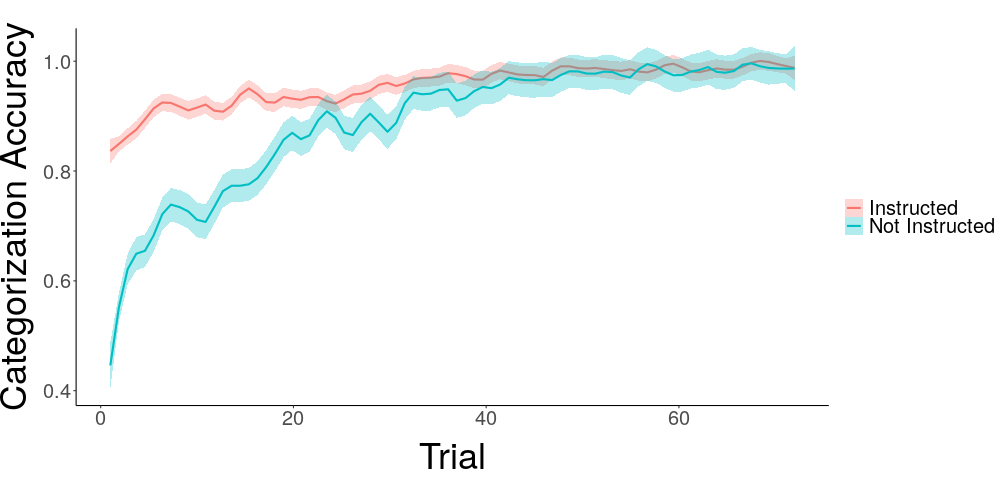
\includegraphics[width=0.5\textwidth]{learning.png}
  \caption{Learning curves for participants in the practiced
    condition.}
  \label{fig:learning}
\end{figure}

\noindent\textbf{Test Phase }
%\subsection*{Memory Performance}
%\label{results:memory}

As outcome variables during the testing phase, we measured reaction
time (RT), hits, and false alarms (FAs), as well as individual
estimates of sensitivity ($d'$) and bias ($C$) under signal detection
theory. To examine the effects of the Learned category, the
Not-Learned category, Practice, and Instruction on these variables, we
employed 2 (Learned: yes vs. no) x 2 (Not-Learned: yes vs. no) x 2
(Practiced: yes vs. no) x 2 (Instructed: yes vs. no) mixed-effect
models with random intercepts for each subject. For hits and FAs, we
employed logistic mixed effect models of the same structure using the
logit link function.

For RT, we found a significant interaction between Instructed and
Not-Learned, $t(37830) = 2.253$, $p = .02$. \textbf{Post-hoc tests?}
Additionally, there was a near-significant interaction between
Instructed and Learned, $t(37830) = 1.672$, $p = .09$, and a
near-significant three-way interaction between Instructed, Learned,
and Not-Learned, $t(37830) = -1.923$, $p = .054$. \textbf{Post-hoc
  tests?}

Looking at hits, we found that flowers in the Learned category were
recollected more frequently than flowers not in the Learned category,
$z = 3.03$, $OR = 1.34$, $p = .002$. Additionally, there was a
near-significant main effect of Not-Learned, such that flowers in the
Not-Learned category were more likely to be remembered, $z = 1.70$,
$OR = 1.18$, $p = .09$. For FAs, we again found that lures in the
Learned category were also more likely to be falsely recollected, $z =
3.92$, $OR = 1.30$, $p < .001$. There was also a significant
interaction between Not-Learned and Instructed, $z = -1.99$, $OR =
0.83$, $p = .04$, and a significant three-way interaction between
Not-Learned, Instructed, and Practiced, $z = 2.13$, $OR = 1.34$, $p =
.03$. \textbf{Post-hoc tests?}

We found no significant effects in the mixed-effects model with regard
to any of our manipulations on sensitivity ($d'$). However,
participants had a lower response bias ($C$) for flowers in the
Learned category than for flowers not in the Learned category,
$t(2130) = -2.00$, $p = .046$. We also observed a significant
interaction between Learned and Not-Learned, $t(2130) = 1.98$, $p =
.048$. \textbf{Post-hoc tests?}

\section*{Discussion}
\label{discussion}
In this study we aimed to discover how different forms of learning
impact schema formation and deployment. To do so, we tested
participant's memory after learning simple rule-based categories under
different learning constraints (practice only, instruction only, both,
neither). Largely, we found little behavioral difference between these
groups, suggesting that they may be equally effective with regard to
forming lasting schemas. However, we did find that the Learned
category had a significant impact on hits, FAs, and response bias
($C$), supporting the idea that all of these forms of category
learning produce representations that are synonymous with schemas
\textbf{(CITE)}.

Future work in this area could reveal boundary conditions in which the
representations produced under these different learning constraints
are dissociable. There is good reason to suspect that such boundary
conditions will exist--- under the recent perspective that category
learning recruits multiple memory systems depending on the category's
nature and the circumstances of learning, we would expect that
practice with immediate feedback would produce more striatal learning,
whereas explicit instruction would result in rule-based learning
invoking the hippocampus and prefrontal cortex \cite{Ashby2011}. We
would then predict a corresponding double-dissociation between
category learning impairment in Parkinson's patients and medial
temporal lobe amnesiacs. Because this paradigm allows for testing the
memory effects of newly-learned categories independently of the
perceptual or statistical features of the stimuli, we believe that it
would be fertile ground for testing this hypothesis in fMRI.

\begin{acknowledgements}
\end{acknowledgements}

\bibliographystyle{spbasic} \bibliography{category_learning}

\end{document}

